\newpage

\section{Ход работы}

\subsection{Определение опорного спектра эрбиевого усилителя}
Для получения опорного спектра излучения эрбиевого волоконного усилителя (EDFA, см. Рис. \ref{fig:edfa_amplifier}) была собрана следующая оптическая схема: выход оптического тестера EXFO FOT-600 (см. Рис. \ref{fig:exfo_fot_600}), используемого в качестве источника широкополосного излучения, был соединен со входом EDFA. Выходное излучение усилителя регистрировалось анализатором оптического спектра YOKOGAWA AQ6370C (см. Рис. \ref{fig:yokogawa_aq6370c}).

Целью данного измерения являлось получение спектральной характеристики EDFA в отсутствие исследуемых SMS-структур, для использования в качестве опорного.

Полученная спектральная характеристика излучения EDFA представлена на Рис. \ref{fig:edfa_reference_spectrum}.

\begin{figure}[H]
\centering
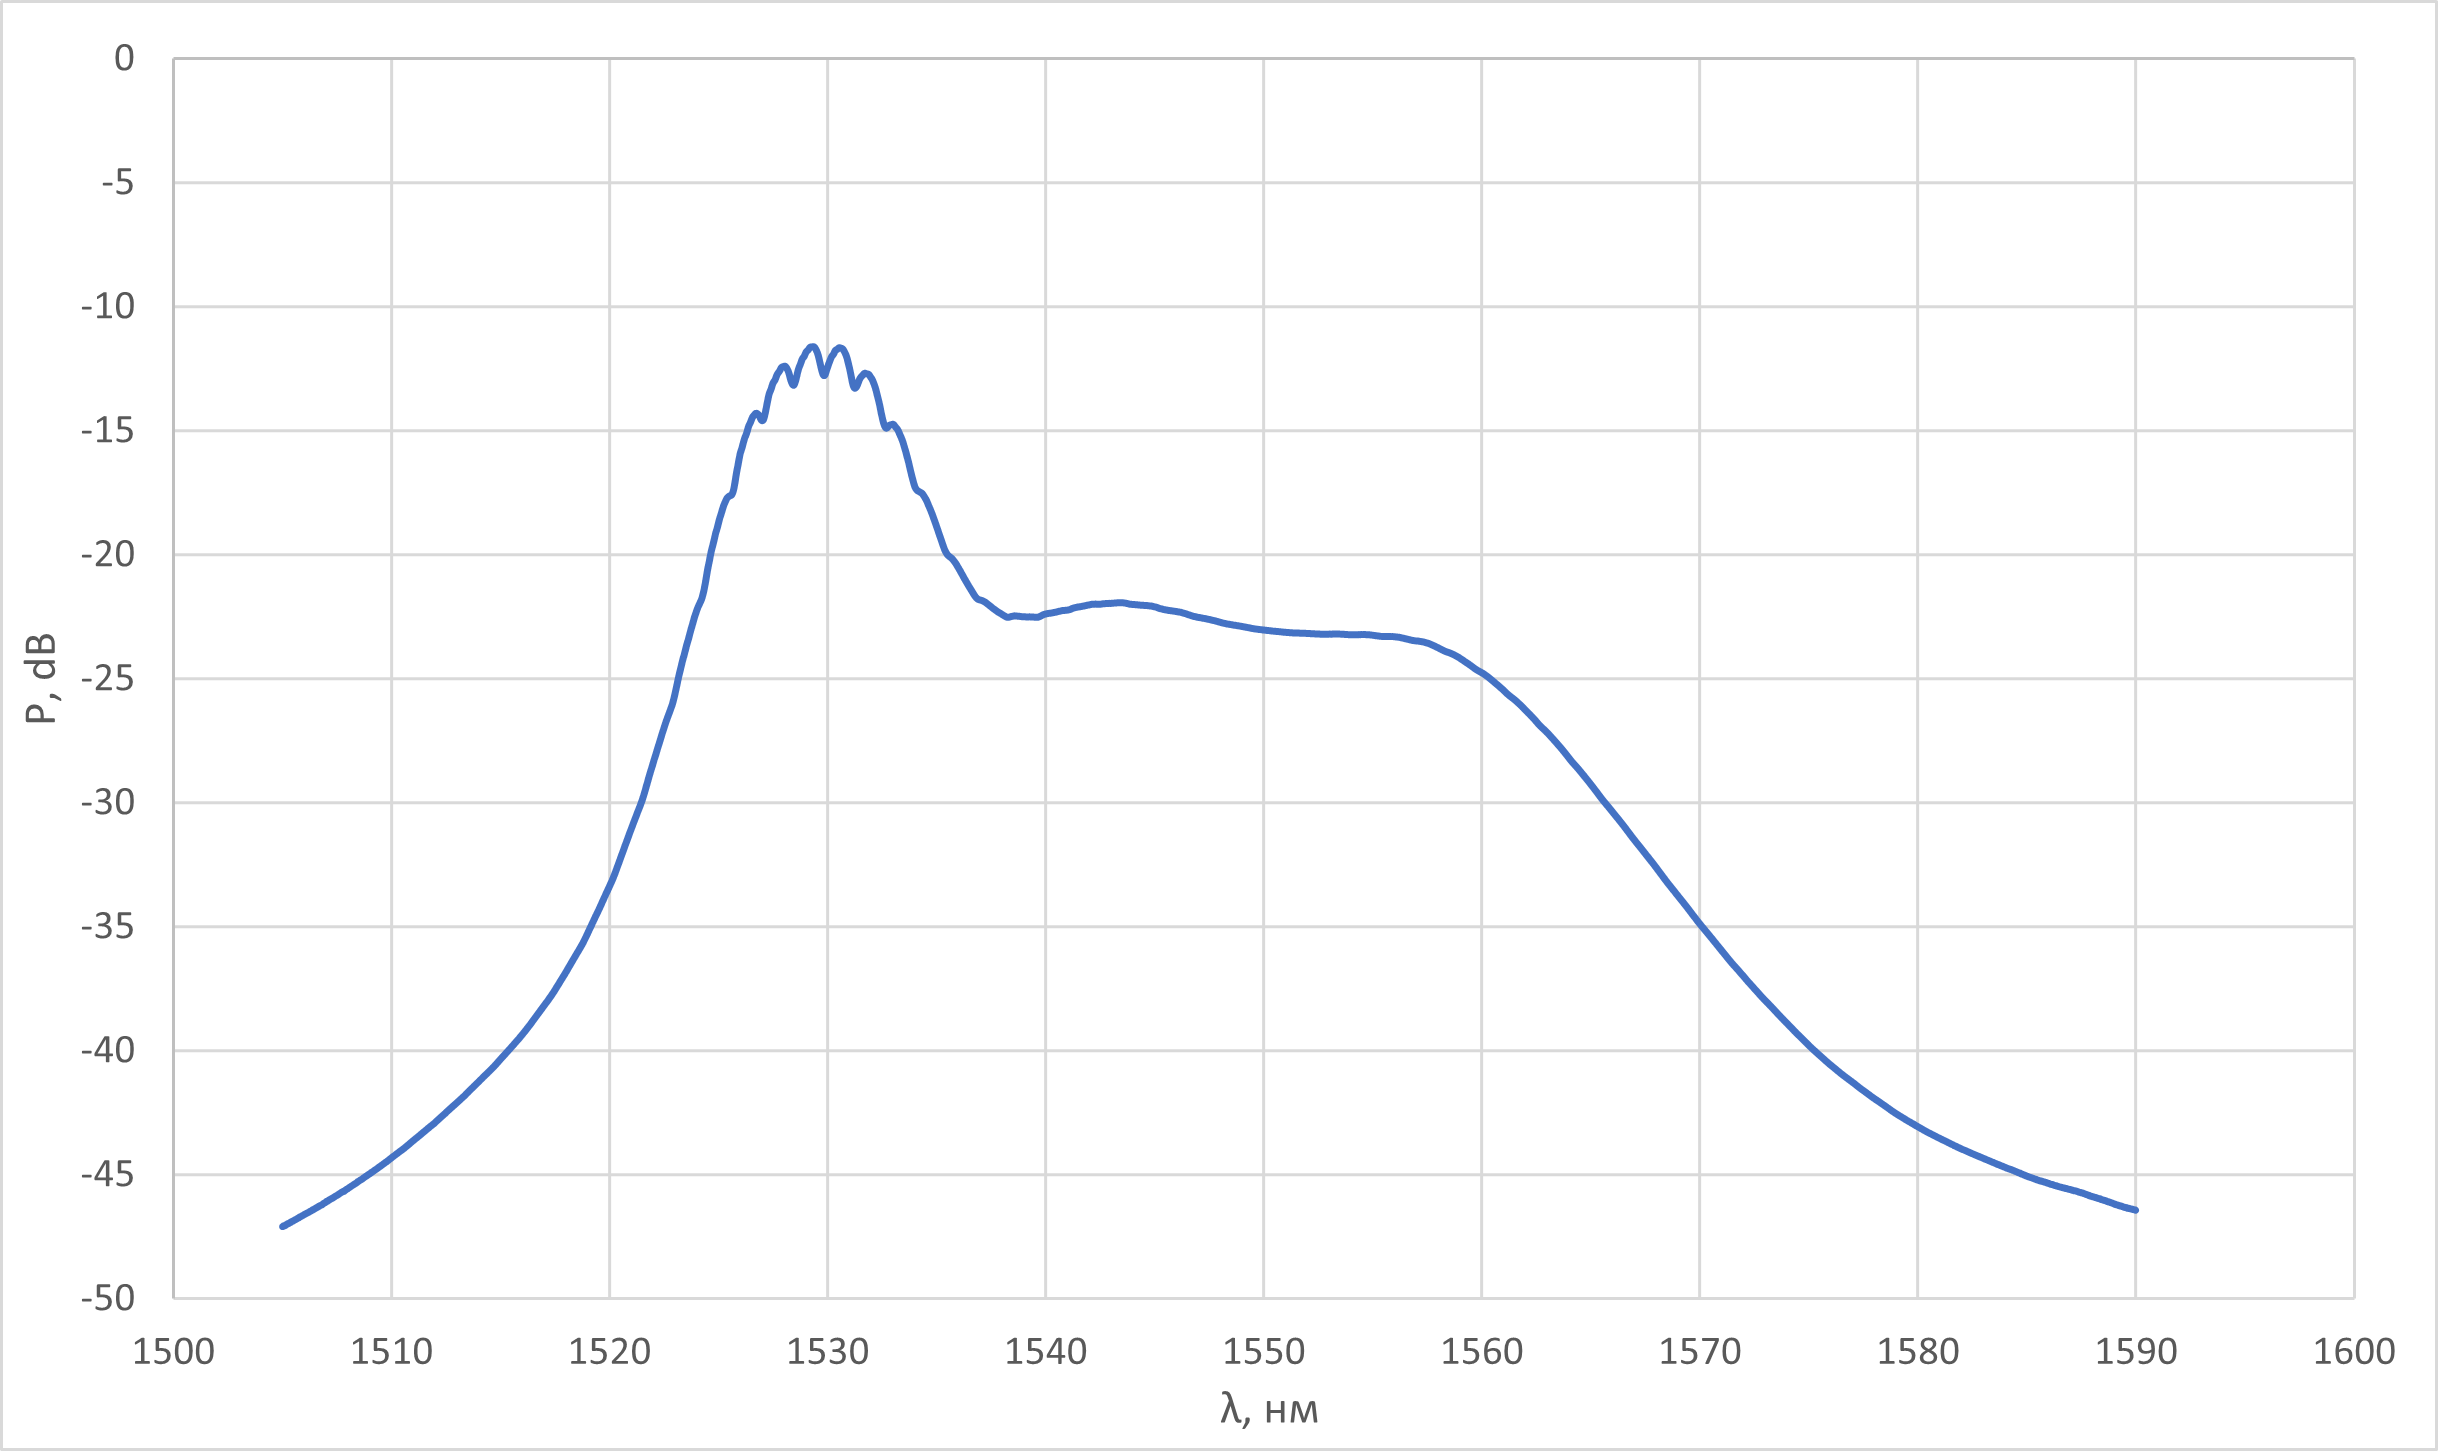
\includegraphics[width=1\textwidth]{pictures/edfa_reference_spectrum.png}
\caption{Опорный спектр излучения эрбиевого усилителя (EDFA)}
\label{fig:edfa_reference_spectrum}
\end{figure}

\subsection{Исследование датчика SMS длиной 4.97 см}
Вторым этапом эксперимента являлось исследование спектральных характеристик волоконного датчика деформации типа SMS (одномод-многомод-одномод) с длиной многомодовой секции $L_{MMF} = 4.97$ см. Датчик был включен в измерительную схему между эрбиевым усилителем (EDFA) и анализатором оптического спектра (OSA). Один конец SMS-датчика был жестко зафиксирован, а к другому концу последовательно прилагались грузы массой от 50 г до 200 г с шагом 50 г (см. Рис. \ref{fig:sms_sensor_mounted} и Рис. \ref{fig:calibration_weights}). Для каждой приложенной массы регистрировался спектр пропускания датчика. Особое внимание уделялось смещению положений минимумов (провалов) в спектре, так как именно их сдвиг характеризует реакцию датчика на деформацию.

На Рис. \ref{fig:sms_4_97_cm_spectra} представлены графики спектра пропускания датчика для различных значений приложенной массы. Видно характерное смещение положений минимумов спектра при увеличении нагрузки.

\begin{figure}[H]
\centering
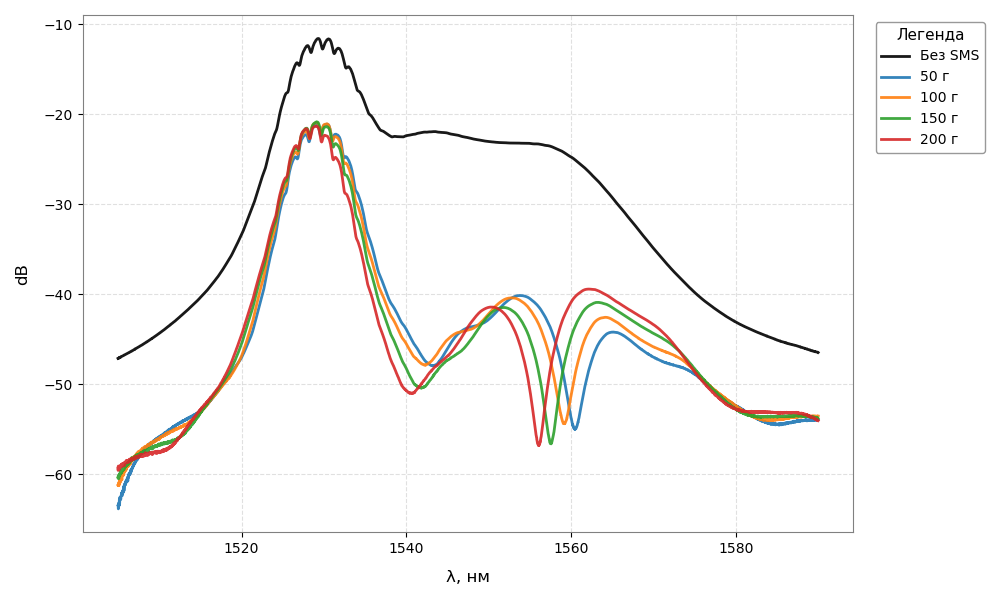
\includegraphics[width=1\textwidth]{pictures/sms_4_97_cm_spectra.png}
\caption{Спектры пропускания датчика SMS ($L_{MMF} = 4.97$ см) для различных приложенных масс.}
\label{fig:sms_4_97_cm_spectra}
\end{figure}

Для более точного определения положений минимумов и отслеживания их сдвига был построен разностный график спектральных характеристик (Рис. \ref{fig:sms_4_97_cm_difference}), который наглядно демонстрирует смещение провалов при изменении нагрузки.

\begin{figure}[H]
\centering
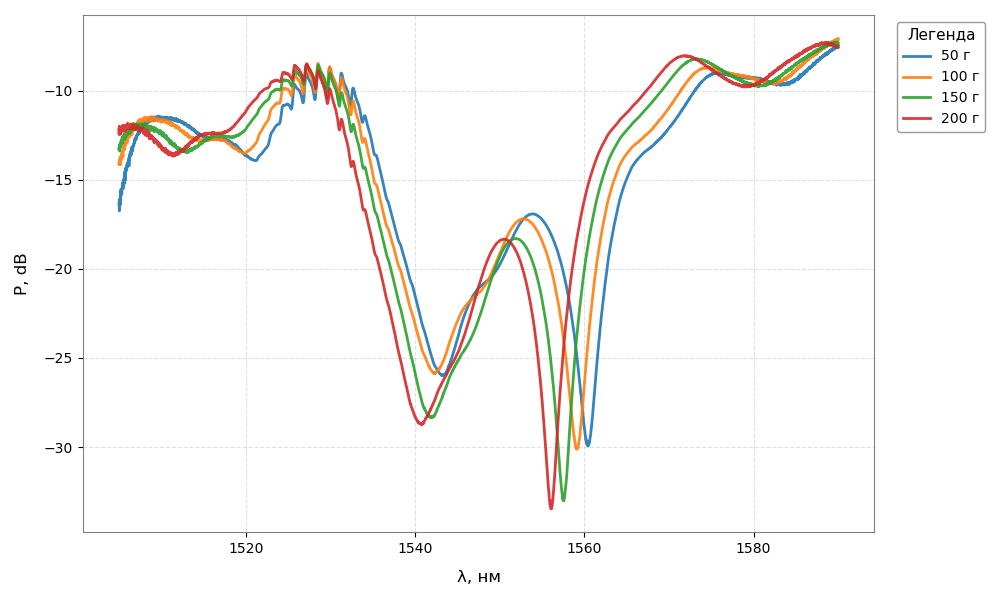
\includegraphics[width=1\textwidth]{pictures/sms_4_97_cm_difference.png}
\caption{Разностный спектр пропускания датчика SMS ($L_{MMF} = 4.97$ см) для определения сдвига минимумов.}
\label{fig:sms_4_97_cm_difference}
\end{figure}

Результаты измерений положений двух характерных минимумов спектра пропускания в зависимости от приложенной массы представлены в Таблице \ref{tab:sms_4_97_cm_data}.

\begin{longtable}[c]{|c|c|c|}
    \caption{Зависимость длин волн минимумов спектра пропускания датчика SMS ($L_{MMF} = 4.97$ см) от массы приложенного груза}
    \label{tab:sms_4_97_cm_data}\\
    \hline
    \rowcolor[HTML]{32CB00} 
    m, г & $\lambda_1$, нм      & $\lambda_2$, нм      \\ \hline
    \endfirsthead
    %
    \endhead
    %
    \rowcolor[HTML]{FFFFFF} 
    50   & 1543.2 & 1560.5 \\ \hline
    \rowcolor[HTML]{FFFFFF} 
    100  & 1542.3 & 1559.1 \\ \hline
    \rowcolor[HTML]{FFFFFF} 
    150  & 1541.9 & 1557.6 \\ \hline
    \rowcolor[HTML]{FFFFFF} 
    200  & 1540.7 & 1556.1 \\ \hline
    \end{longtable}

На основе полученных данных были построены графики зависимости длины волны минимумов от приложенной массы (Рис. \ref{fig:sms_4_97_cm_plot}). Графики демонстрируют линейное смещение длин волн минимумов в коротковолновую область с увеличением нагрузки.

\begin{figure}[H]
\centering
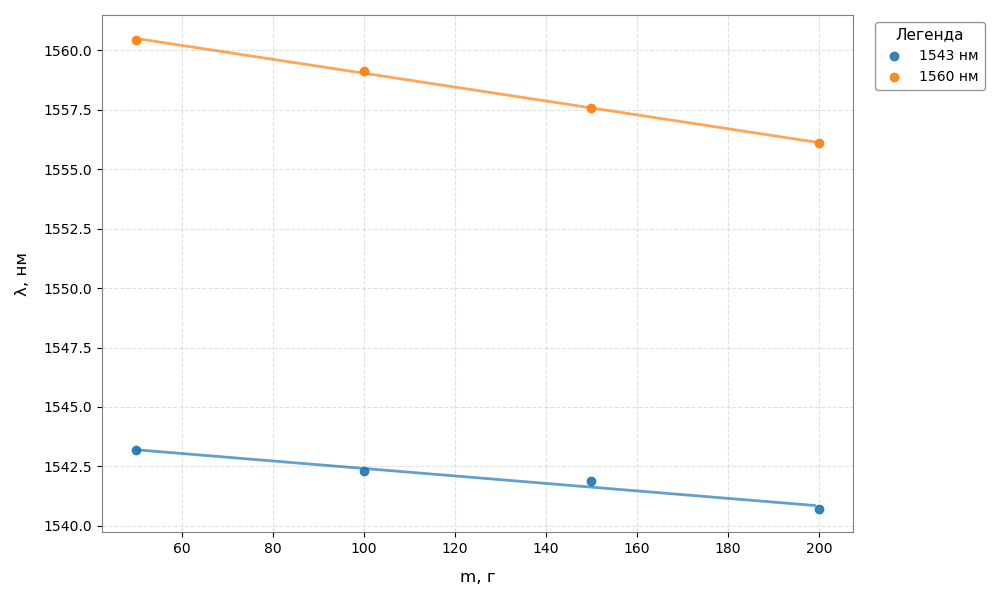
\includegraphics[width=1\textwidth]{pictures/sms_4_97_cm_plot.png}
\caption{Зависимость длин волн минимумов спектра пропускания датчика SMS ($L_{MMF} = 4.97$ см) от массы приложенного груза. }
\label{fig:sms_4_97_cm_plot}
\end{figure}

\subsection{Исследование датчика SMS длиной 10.2 см}
Аналогичные измерения были проведены для датчика SMS с длиной многомодовой секции $L_{MMF} = 10.2$ см. К датчику прилагались грузы массой от 50 г до 300 г с шагом 50 г. 

На Рис. \ref{fig:sms_10_2_cm_spectra} представлены графики спектра пропускания датчика для различных значений приложенной массы.

\begin{figure}[H]
\centering
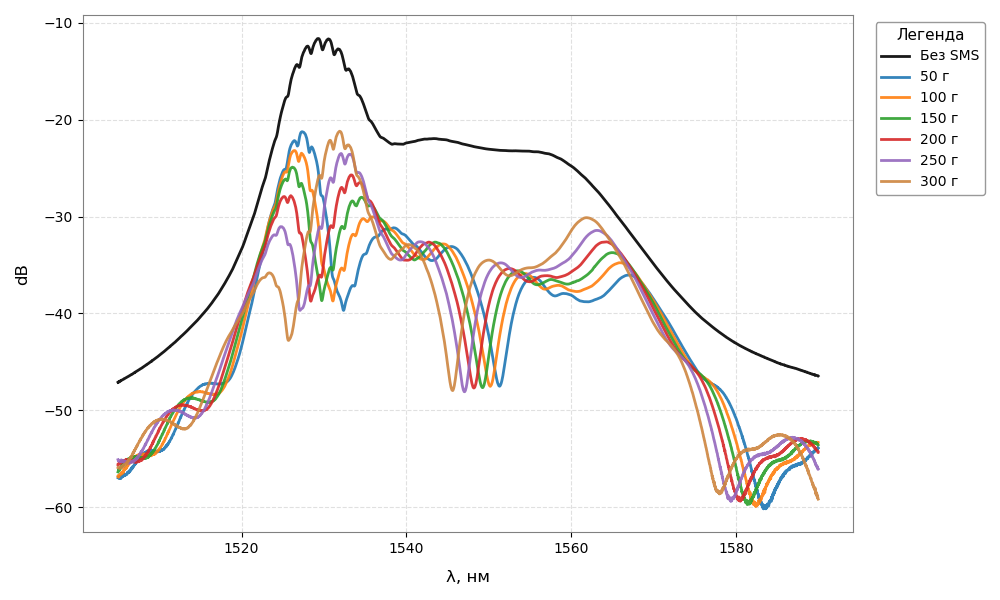
\includegraphics[width=1\textwidth]{pictures/sms_10_2_cm_spectra.png}
\caption{Спектры пропускания датчика SMS ($L_{MMF} = 10.2$ см) для различных приложенных масс.}
\label{fig:sms_10_2_cm_spectra}
\end{figure}

Аналогично был построен разностный график спектральных характеристик (Рис. \ref{fig:sms_10_2_cm_difference}).

\begin{figure}[H]
\centering
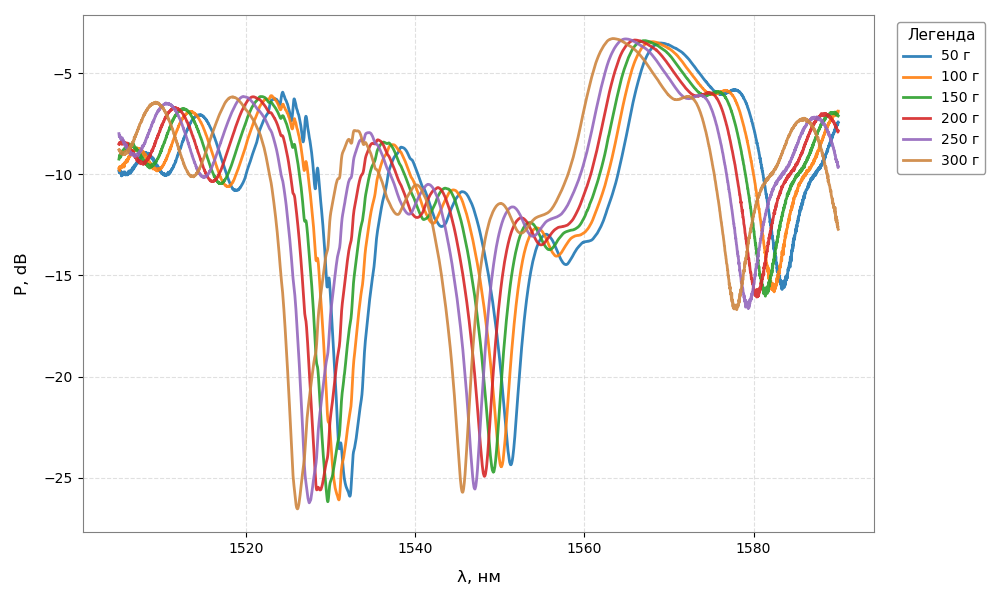
\includegraphics[width=1\textwidth]{pictures/sms_10_2_cm_difference.png}
\caption{Разностный спектр пропускания датчика SMS ($L_{MMF} = 10.2$ см) для определения сдвига минимумов.}
\label{fig:sms_10_2_cm_difference}
\end{figure}

Результаты измерений положений шести характерных минимумов спектра пропускания в зависимости от приложенной массы представлены в Таблице \ref{tab:sms_10_2_cm_data}.

\begin{longtable}[c]{|c|c|c|c|c|c|c|}
    \caption{Зависимость длин волн минимумов спектра пропускания датчика SMS ($L_{MMF} = 10.2$ см) от массы приложенного груза}
    \label{tab:sms_10_2_cm_data}\\
    \hline
    \rowcolor[HTML]{32CB00} 
    m, г & $\lambda_1$, нм      & $\lambda_2$, нм      & $\lambda_3$, нм      & $\lambda_4$, нм      & $\lambda_5$, нм      & $\lambda_6$, нм      \\ \hline
    \endfirsthead
    %
    \endhead
    %
    \rowcolor[HTML]{FFFFFF} 
    50   & 1518.9 & 1532.3 & 1543.1 & 1551.3 & 1557.8 & 1583.4 \\ \hline
    \rowcolor[HTML]{FFFFFF} 
    100  & 1517.9 & 1531.0 & 1542.2 & 1550.2 & 1556.7 & 1582.4 \\ \hline
    \rowcolor[HTML]{FFFFFF} 
    150  & 1517.1 & 1529.7 & 1541.0 & 1549.2 & 1555.8 & 1581.4 \\ \hline
    \rowcolor[HTML]{FFFFFF} 
    200  & 1516.0 & 1528.8 & 1540.3 & 1548.2 & 1554.9 & 1580.4 \\ \hline
    \rowcolor[HTML]{FFFFFF} 
    250  & 1514.9 & 1527.5 & 1539.3 & 1547.1 & 1553.8 & 1579.4 \\ \hline
    \rowcolor[HTML]{FFFFFF} 
    300  & 1513.8 & 1526.1 & 1537.9 & 1545.6 & 1552.5 & 1578.0 \\ \hline
    \end{longtable}

Графики зависимости длин волн минимумов от приложенной массы для датчика $L_{MMF} = 10.2$ см представлены на Рис. \ref{fig:sms_10_2_cm_plot}. Наблюдается аналогичная линейная зависимость сдвига минимумов от нагрузки.

\begin{figure}[H]
\centering
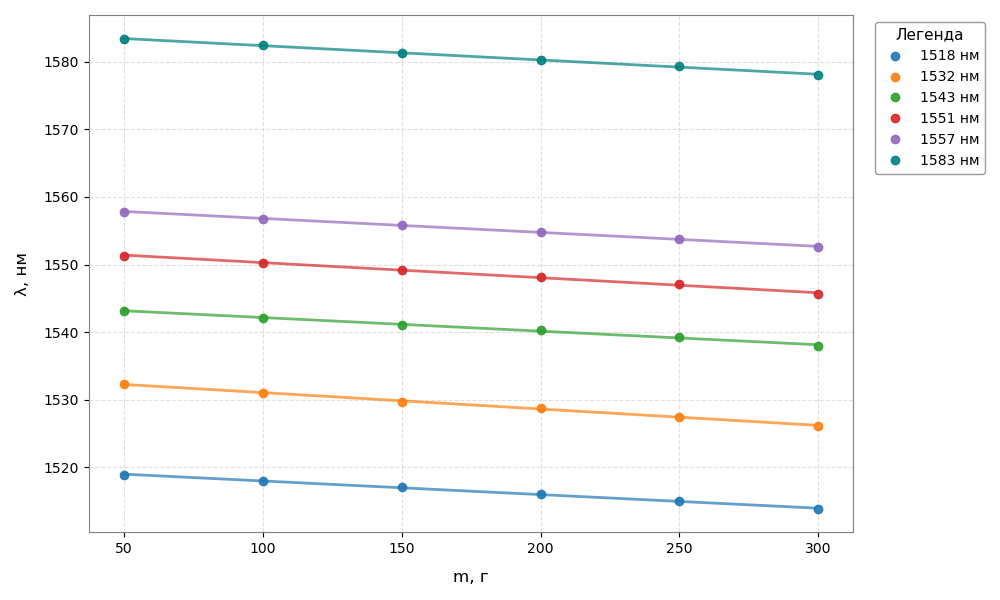
\includegraphics[width=1\textwidth]{pictures/sms_10_2_cm_plot.png}
\caption{Зависимость длин волн минимумов спектра пропускания датчика SMS ($L_{MMF} = 10.2$ см) от массы приложенного груза. }
\label{fig:sms_10_2_cm_plot}
\end{figure}

\subsection{Исследование датчика SMS длиной 20.5 см}
Третий исследуемый датчик SMS имел длину многомодовой секции $L_{MMF} = 20.5$ см. Нагрузка варьировалась от 50 г до 300 г с шагом 50 г. 

На Рис. \ref{fig:sms_20_5_cm_spectra} представлены графики спектра пропускания датчика для различных значений приложенной массы.

\begin{figure}[H]
\centering
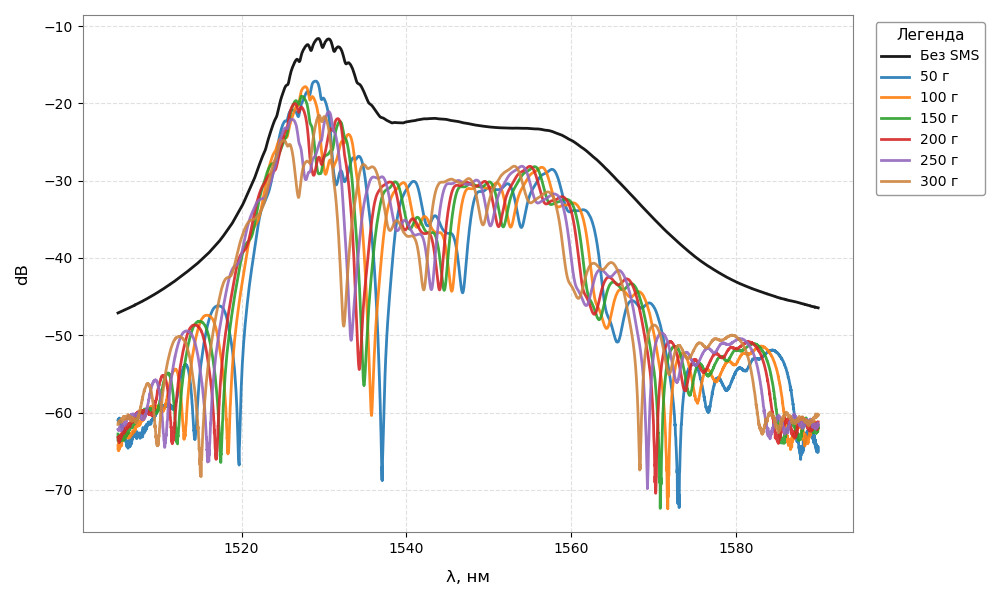
\includegraphics[width=1\textwidth]{pictures/sms_20_5_cm_spectra.png}
\caption{Спектры пропускания датчика SMS ($L_{MMF} = 20.5$ см) для различных приложенных масс.}
\label{fig:sms_20_5_cm_spectra}
\end{figure}

Тоже был построен разностный график спектральных характеристик (Рис. \ref{fig:sms_20_5_cm_difference}).

\begin{figure}[H]
\centering
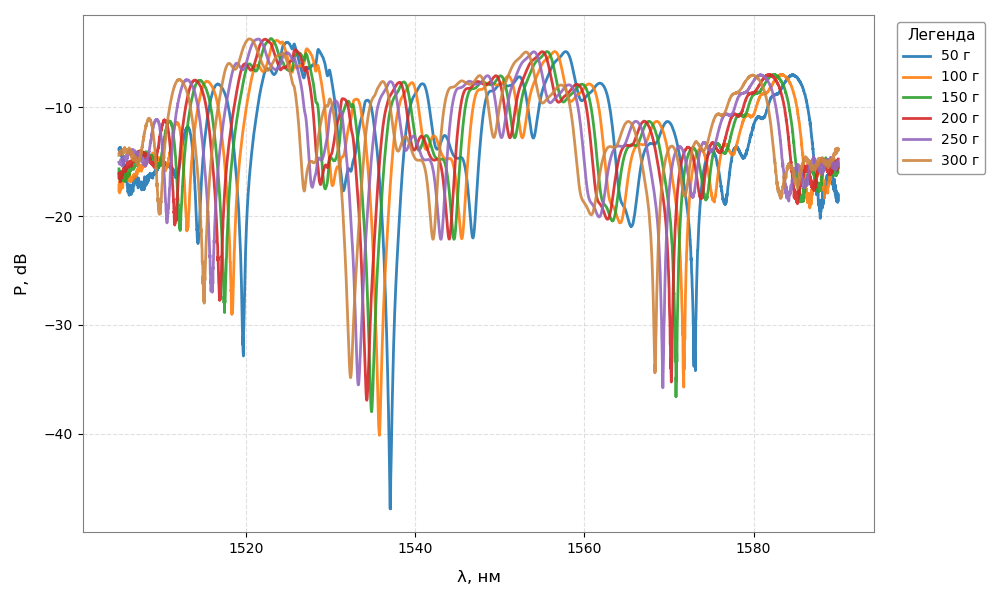
\includegraphics[width=1\textwidth]{pictures/sms_20_5_cm_difference.png}
\caption{Разностный спектр пропускания датчика SMS ($L_{MMF} = 20.5$ см) для определения сдвига минимумов.}
\label{fig:sms_20_5_cm_difference}
\end{figure}

Результаты измерений положений двенадцати характерных минимумов спектра пропускания в зависимости от приложенной массы представлены в Таблице \ref{tab:sms_20_5_cm_data}.

\begin{longtable}[c]{|c|c|c|c|c|c|c|}
    \caption{Зависимость длин волн минимумов спектра пропускания датчика SMS ($L_{MMF} = 20.5$ см) от массы приложенного груза}
    \label{tab:sms_20_5_cm_data}\\
    \hline
    \rowcolor[HTML]{32CB00} 
    m, г & $\lambda_1$, нм      & $\lambda_2$, нм      & $\lambda_3$, нм      & $\lambda_4$, нм     & $\lambda_5$, нm      & $\lambda_6$, нм      \\ \hline
    \endfirsthead
    %
    \endhead
    %
    50   & 1514.3 & 1519.7 & 1526.9 & 1531.5 & 1537.1 & 1546.8 \\ \hline
    100  & 1513.0 & 1518.3 & 1525.5 & 1530.2 & 1535.8 & 1545.5 \\ \hline
    150  & 1512.2 & 1517.5 & 1525.2 & 1529.4 & 1534.9 & 1544.6 \\ \hline
    200  & 1511.6 & 1516.9 & 1524.1 & 1528.8 & 1534.3 & 1544.0 \\ \hline
    250  & 1510.7 & 1516.0 & 1523.5 & 1527.8 & 1533.3 & 1543.0 \\ \hline
    300  & 1509.8 & 1515.1 & 1522.6 & 1526.9 & 1532.4 & 1542.1 \\ \hline
    \end{longtable}

    \begin{longtable}[c]{|c|c|c|c|c|c|c|}
        \hline
        \rowcolor[HTML]{32CB00} 
        m, г & $\lambda_7$, нм      & $\lambda_8$, нм      & $\lambda_9$, нm      & $\lambda_{10}$, нм     & $\lambda_{11}$, нm     & $\lambda_{12}$, нм     \\ \hline
        \endfirsthead
        %
        \endhead
        %
        50   & 1554.0 & 1559.7 & 1565.5 & 1573.1 & 1576.7 & 1587.9 \\ \hline
        100  & 1552.7 & 1558.4 & 1564.2 & 1571.7 & 1575.4 & 1586.6 \\ \hline
        150  & 1551.8 & 1557.5 & 1563.3 & 1570.8 & 1574.4 & 1585.5 \\ \hline
        200  & 1551.2 & 1557.0 & 1562.7 & 1570.3 & 1573.8 & 1585.2 \\ \hline
        250  & 1550.2 & 1555.9 & 1561.8 & 1569.3 & 1572.8 & 1584.2 \\ \hline
        300  & 1549.3 & 1555.1 & 1560.8 & 1568.3 & 1571.9 & 1583.2 \\ \hline
        \end{longtable}

Графики зависимости длин волн минимумов от приложенной массы для датчика $L_{MMF} = 20.5$ см представлены на Рис. \ref{fig:sms_20_5_cm_plot}. Как и для предыдущих датчиков, наблюдается линейная зависимость сдвига минимумов от нагрузки.

\begin{figure}[H]
\centering
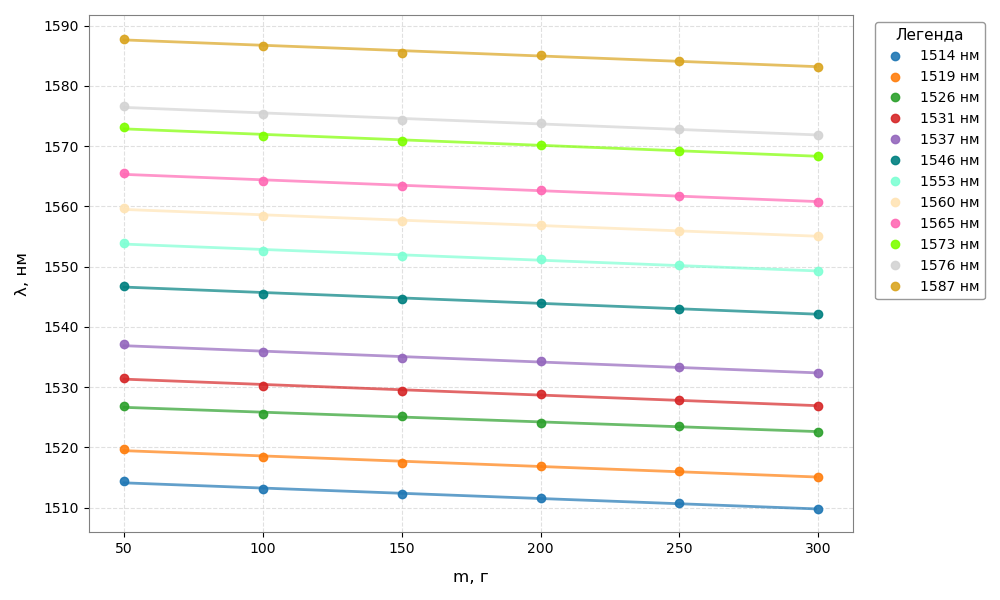
\includegraphics[width=1\textwidth]{pictures/sms_20_5_cm_plot.png}
\caption{Зависимость длин волн минимумов спектра пропускания датчика SMS ($L_{MMF} = 20.5$ см) от массы приложенного груза. }
\label{fig:sms_20_5_cm_plot}
\end{figure}

\subsection{Анализ чувствительности датчиков SMS к продольному растяжению}
Для количественной оценки чувствительности исследованных SMS-датчиков к продольному растяжению, вызванному приложенной массой, для каждого отслеживаемого минимума спектра пропускания была проведена линейная аппроксимация зависимости его длины волны $\lambda$ от массы груза $m$:
\begin{equation}
    \lambda(m) = k \cdot m + \lambda_0
    \label{eq:linear_approximation_lambda_m}
\end{equation}
Коэффициент наклона $k = \frac{\Delta \lambda}{\Delta m}$ характеризует чувствительность датчика по данному минимуму к изменению массы и измеряется в нм/г. Коэффициенты $k$ и их погрешности $\Delta k$ рассчитывались с использованием метода наименьших квадратов (МНК).

В Таблице \ref{tab:sms_sensitivity_summary} сведены экспериментально определенные коэффициенты, характеризующие зависимость длины волны минимумов спектра пропускания от приложенной нагрузки и относительного удлинения для датчиков SMS различной длины.


\begin{longtable}[c]{|c|
    >{\columncolor[HTML]{FFFFFF}}c |c|c|c|c|}
    \caption{Сводная таблица чувствительности датчиков SMS к растяжению для различных длин многомодовой секции $L_{MMF}$}
    \label{tab:sms_sensitivity_summary}\\
    \hline
    \cellcolor[HTML]{32CB00}$L_{MMF}$,   см &
      \cellcolor[HTML]{32CB00}$\lambda$, нм &
      \cellcolor[HTML]{32CB00}$\Delta\lambda/\Delta   m$, нм/100г &
      \cellcolor[HTML]{32CB00}$\sigma$,   нм/100г &
      \cellcolor[HTML]{32CB00}$\Delta\lambda/\Delta\varepsilon$,   нм/1\% &
      \cellcolor[HTML]{32CB00}$\sigma$, нм/1\% \\ \hline
    \endfirsthead
    \endhead
                            & 1518 & -1.57 & -0.14 & -15.7 & -1.4 \\ \cline{2-6} 
    \multirow{-2}{*}{4.97}  & 1532 & -2.92 & -0.04 & -29.2 & -0.4 \\ \hline
                            & 1543 & -2.02 & -0.04 & -20.2 & -0.4 \\ \cline{2-6} 
                            & 1551 & -2.43 & -0.05 & -24.3 & -0.5 \\ \cline{2-6} 
                            & 1557 & -2.02 & -0.06 & -20.2 & -0.6 \\ \cline{2-6} 
                            & 1583 & -2.23 & -0.06 & -22.3 & -0.6 \\ \cline{2-6} 
                            & 1543 & -2.07 & -0.05 & -20.7 & -0.5 \\ \cline{2-6} 
    \multirow{-6}{*}{10.2}  & 1560 & -2.12 & -0.05 & -21.2 & -0.5 \\ \hline
                            & 1514 & -1.74 & -0.07 & -17.4 & -0.7 \\ \cline{2-6} 
                            & 1519 & -1.75 & -0.08 & -17.5 & -0.8 \\ \cline{2-6} 
                            & 1526 & -1.61 & -0.09 & -16.1 & -0.9 \\ \cline{2-6} 
                            & 1531 & -1.76 & -0.07 & -17.6 & -0.7 \\ \cline{2-6} 
                            & 1537 & -1.81 & -0.07 & -18.1 & -0.7 \\ \cline{2-6} 
                            & 1546 & -1.8  & -0.07 & -18   & -0.7 \\ \cline{2-6} 
                            & 1553 & -1.79 & -0.07 & -17.9 & -0.7 \\ \cline{2-6} 
                            & 1560 & -1.78 & -0.07 & -17.8 & -0.7 \\ \cline{2-6} 
                            & 1565 & -1.81 & -0.07 & -18.1 & -0.7 \\ \cline{2-6} 
                            & 1573 & -1.82 & -0.08 & -18.2 & -0.8 \\ \cline{2-6} 
                            & 1576 & -1.83 & -0.07 & -18.3 & -0.7 \\ \cline{2-6} 
    \multirow{-12}{*}{20.5} & 1587 & -1.78 & -0.1  & -17.8 & -1   \\ \hline
\end{longtable}

Следует отметить, что стандартная чувствительность волоконных датчиков деформации на основе Брэгговских решеток (FBG) составляет порядка 12 нм/\% (взято из исследования от института ИТМО, \url{https://ntv.ifmo.ru/file/article/22357.pdf}), что, согласно данным измерений, несколько меньше чувствительности исследованных SMS-датчиков в данном эксперименте. 

\subsection{Исследование спекл-картин в одномодовом и многомодовом волокнах}
Для визуализации и анализа спекл-картин, формирующихся при распространении когерентного излучения в оптических волокнах различного типа, была собрана экспериментальная установка, включающая лазерный диод с длиной волны излучения 650 нм и исследуемый отрезок оптического волокна (одномодового с диаметром сердцевины 9 мкм и многомодового с диаметром сердцевины 62.5 мкм). Излучение из волокна направлялось на обзорный экран, расположенный на расстоянии 25 см от выходного торца волокна. Формирующаяся на экране спекл-картина фотографировалась для последующего анализа.

Теоретическая оценка количества поддерживаемых мод может быть выполнена на основе V-параметра волокна по формуле $N \approx V^2/2$, где $V = \frac{2\pi a}{\lambda} \sqrt{n_1^2 - n_2^2} = \frac{2\pi a}{\lambda} \cdot NA$. При неизвестной разнице показателей преломления $\Delta n = n_1 - n_2$, но предполагая типичные значения для данного типа волокон (в диапазоне от $0.001$ до $0.01$), было рассчитано возможное число мод. Для одномодового волокна (диаметр сердцевины 9 мкм, $\lambda = 650$ нм) количество мод лежит в диапазоне от $N \approx 2.76$ до $N \approx 27.6$ (для $\Delta n = 0.001$ и $0.01$ соответственно). Для многомодового волокна (диаметр сердцевины 62.5 мкм, $\lambda = 650$ нм) расчетное число мод составляет от $N \approx 133$ до $N \approx 1332$.

Визуальное наблюдение и анализ полученных фотографий спекл-картин показал, что для одномодового волокна наблюдается небольшое количество мод (визуально около 3, LP21), в то время как для многомодового волокна отчетливо видно значительно большее число интерферирующих мод (много больше 10).

Для количественной оценки углового расхождения излучения на выходе волокон был измерен размер спекл-картины на фотографиях, для чего мы использовали масштабную линейку, присутствующую на снимках. Полученный размер пятна на экране был пересчитан в угловое расхождение, учитывая расстояние от торца волокна до экрана (25 см). Для сравнения была рассчитана угловая расходимость, обусловленная дифракцией на апертуре, равной диаметру сердцевины волокна (размер пятна Эйри). Расчеты представлены в Таблице \ref{tab:speckle_comparison}.

\begin{longtable}[c]{|c|c|c|c|c|}
    \caption{Сравнение углового расхождения спекл-картины с размером пятна Эйри}
    \label{tab:speckle_comparison}\\
    \hline
    \rowcolor[HTML]{32CB00}
    d, мкм & $\lambda$, нм & Размер пятна, мм & Угл. расхождение, рад & Пятно Эйри, рад \\ \hline
    \endfirsthead
    %
    \endhead
    %
    9 & 650 & 43 & 0.171 & 0.176 \\ \hline
    62.5 & 650 & 80 & 0.318 & 0.025 \\ \hline
\end{longtable}

Также представлены расчеты теоретического количества мод в зависимости от разницы показателей преломления, сведенные в Таблицу \ref{tab:mode_calculation}.

\begin{longtable}[c]{|c|c|c|c|}
    \caption{Расчет количества мод для различных разностей показателей преломления}
    \label{tab:mode_calculation}\\
    \hline
    \rowcolor[HTML]{32CB00}
    $\Delta n$ & d, мкм & $\lambda$, нм & N \\ \hline
    \endfirsthead
    %
    \endhead
    %
    0.001 & 9 & 650 & 2.8 \\ \hline
    0.01 & 9 & 650 & 28 \\ \hline
    0.001 & 62.5 & 650 & 130 \\ \hline
    0.01 & 62.5 & 650 & 1330 \\ \hline
\end{longtable}

На рисунках (Рис. \ref{fig:speckle_one_mode} и Рис. \ref{fig:speckle_multi_mode}) представлены фотографии спекл-картин, полученные для одномодового и многомодового волокон соответственно.

\begin{figure}[H]
    \centering
    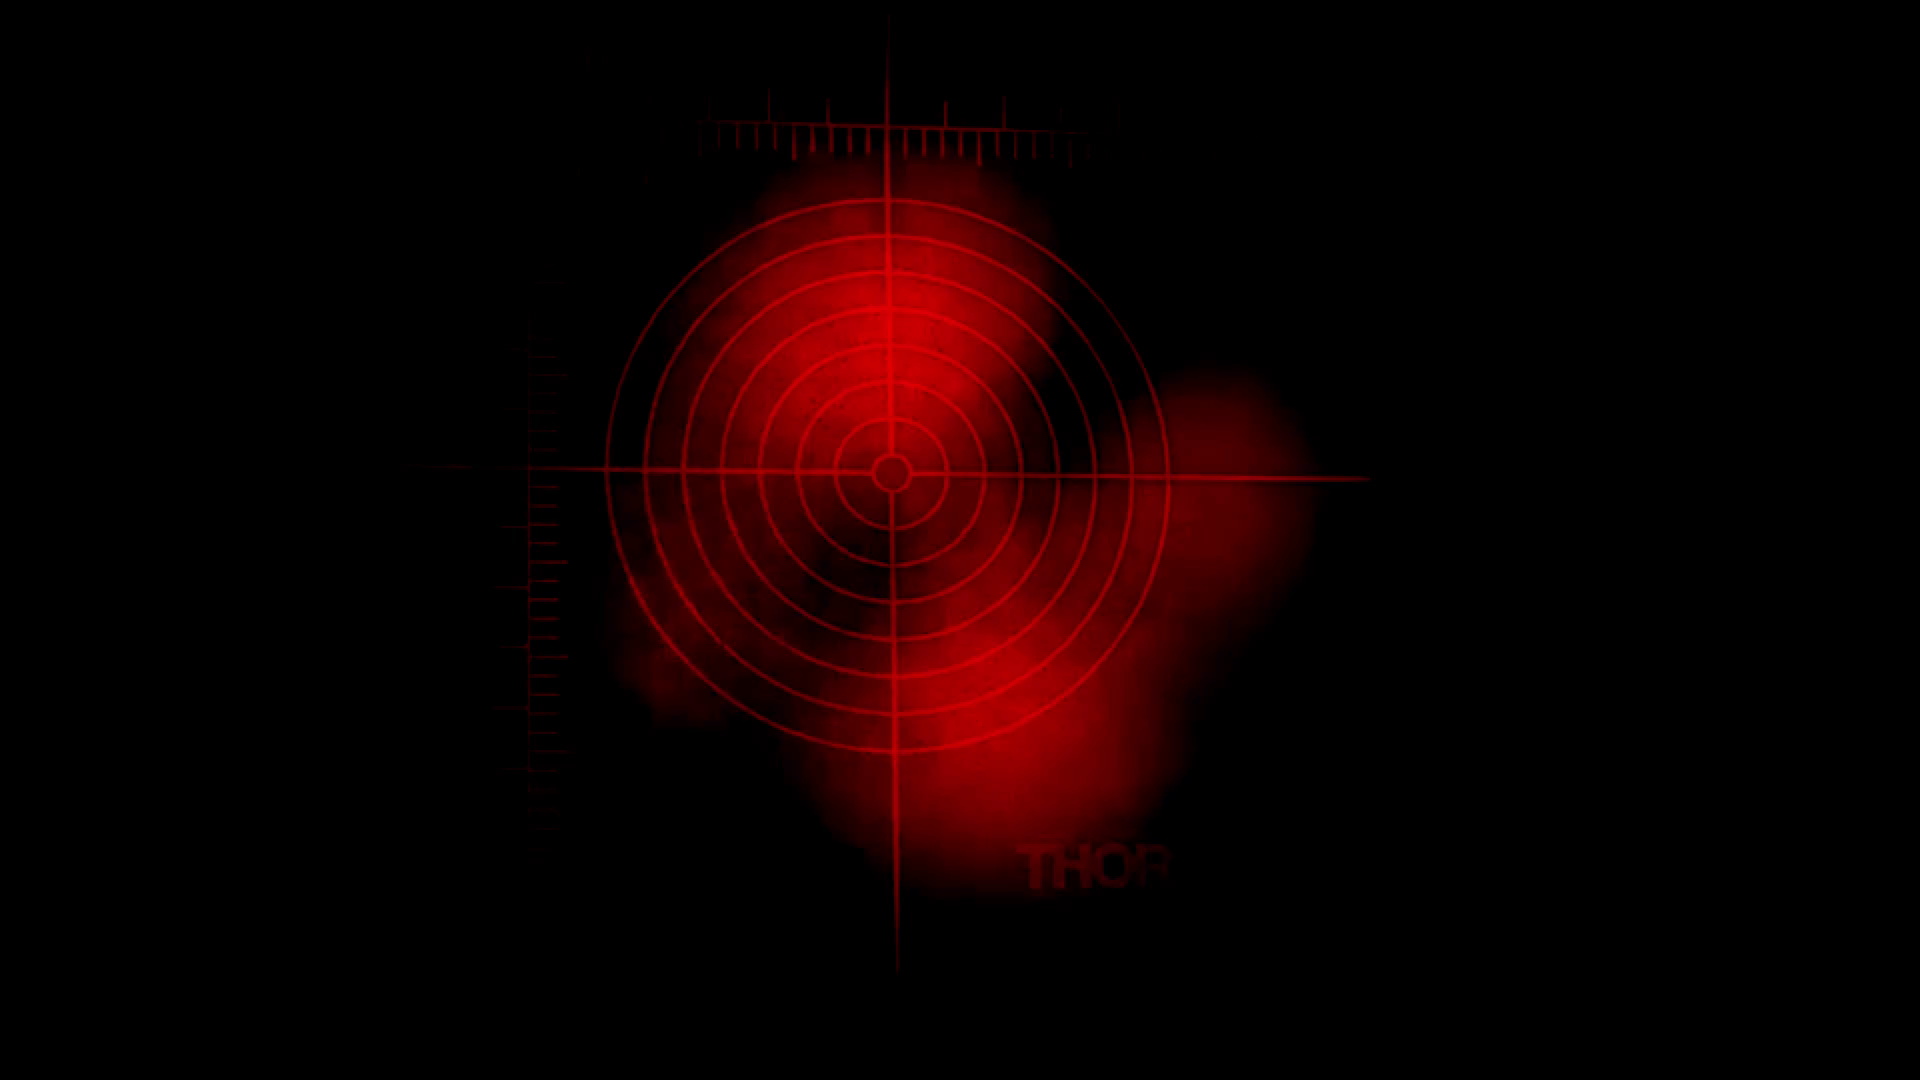
\includegraphics[width=0.8\textwidth]{pictures/speckle_one_mode.png}
    \caption{Спекл-картина для одномодового волокна}
    \label{fig:speckle_one_mode}
\end{figure}

\begin{figure}[H]
    \centering
    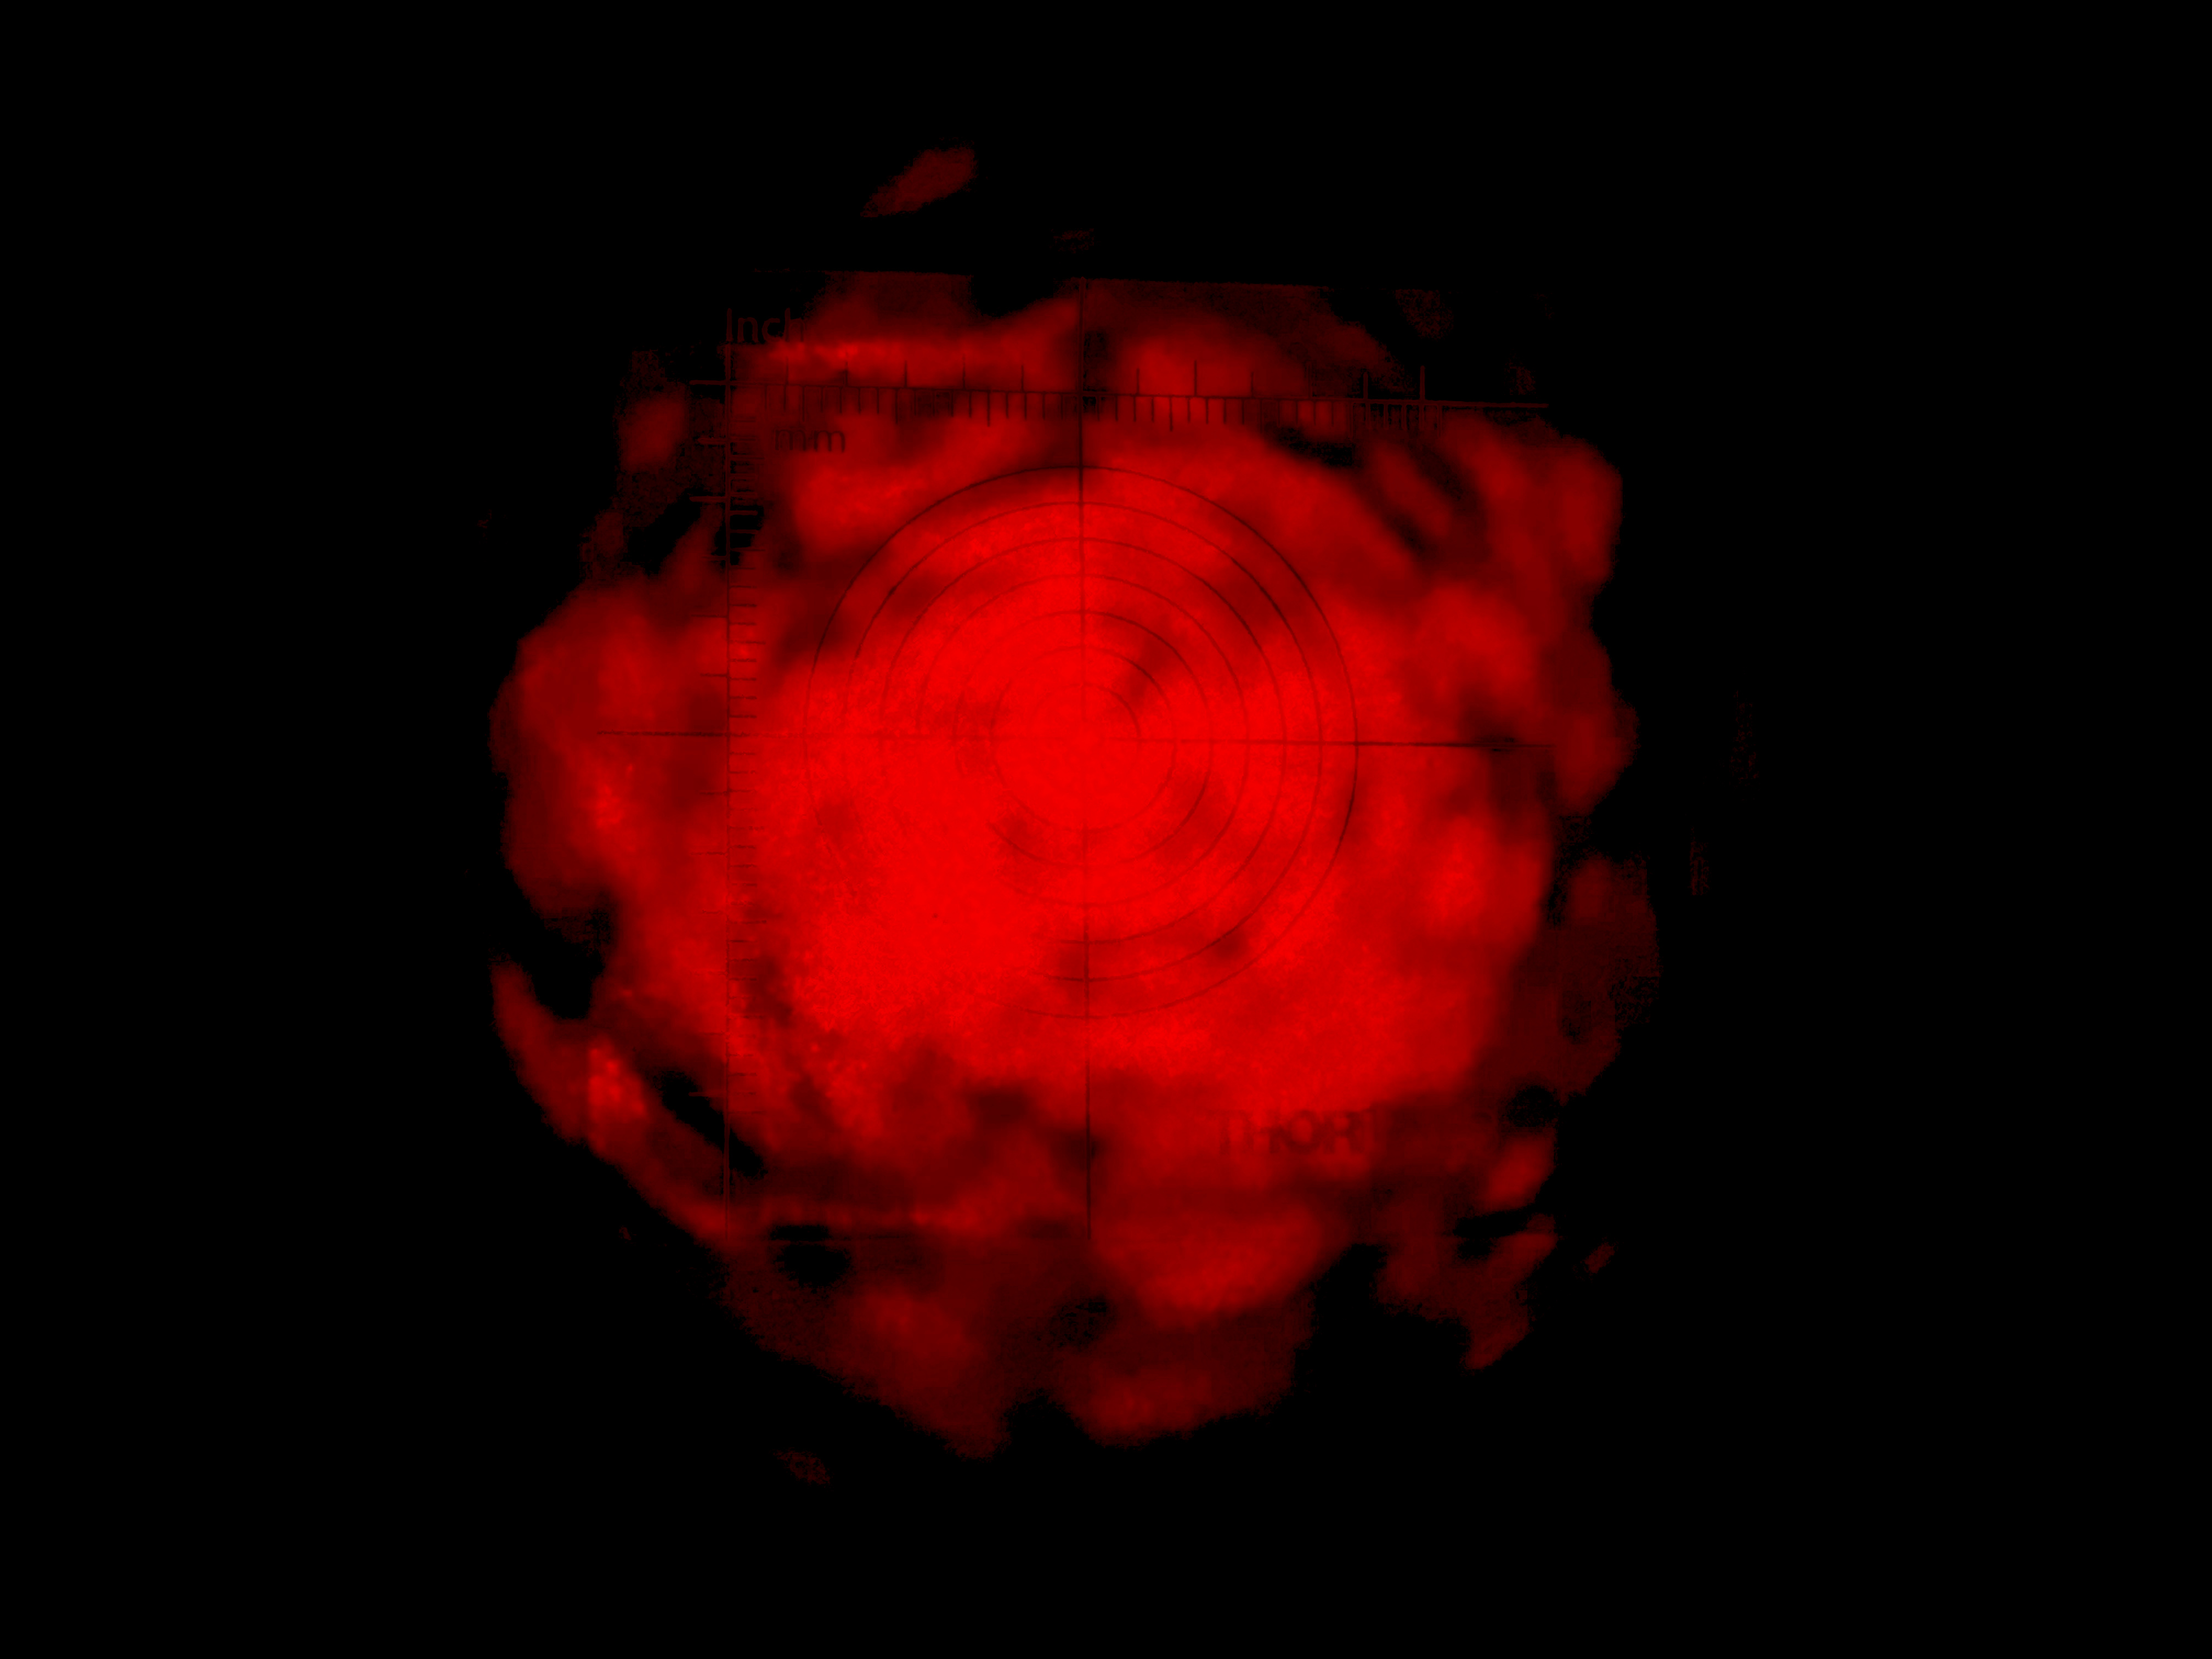
\includegraphics[width=0.8\textwidth]{pictures/speckle_multi_mode.jpg}
    \caption{Спекл-картина для многомодового волокна}
    \label{fig:speckle_multi_mode}
\end{figure}

    